\documentclass[usenames,dvipsnames,pdftex]{beamer}

\mode<presentation> {

% The Beamer class comes with a number of default slide themes
% which change the colors and layouts of slides. Below this is a list
% of all the themes, uncomment each in turn to see what they look like.
\newcommand{\theauthor}[1]{%
\includegraphics[width=0.4\textwidth]{#1}\\#1
}%

%\usetheme{default}
%\usetheme{AnnArbor}
\usetheme{Antibes}
%\usetheme{Bergen}
%\usetheme{Berkeley}
%\usetheme{Berlin}
%\usetheme{Boadilla}                
%\usetheme{CambridgeUS} %kkkkkkkkkkkk
%\usetheme{Copenhagen}
%\usetheme{Darmstadt}  % 22222222222222
%\usetheme{Dresden}
%\usetheme{Frankfurt}
%\usetheme{Goettingen} 
%\usetheme{Hannover} %llllllllllllll
%\usetheme{Ilmenau}
%\usetheme{JuanLesPins}
%\usetheme{Luebeck}
%\usetheme{Madrid} %3333333333333333333
%\usetheme{Malmoe}
%\usetheme{Marburg}
%\usetheme{Montpellier} %2222222
%\usetheme{PaloAlto}
%\usetheme{Pittsburgh}
%\usetheme{Rochester}
%\usetheme{Singapore}
%\usetheme{Szeged} % 0000000000000000
% \usetheme{Warsaw}

% As well as themes, the Beamer class has a number of color themes
% for any slide theme. Uncomment each of these in turn to see how it
% changes the colors of your current slide theme.

%\usecolortheme{albatross}
%\usecolortheme{beaver} % 0000000000
%\usecolortheme{beetle}
%\usecolortheme{crane}
\usecolortheme{dolphin} % 0000000
%\usecolortheme{dove}   %%%%%%%%%%
%\usecolortheme{fly}
%\usecolortheme{lily}
%\usecolortheme{orchid} %%%%%%%%%%%
%\usecolortheme{rose}
%\usecolortheme{seagull}
%\usecolortheme{seahorse}
%\usecolortheme{whale}
%\usecolortheme{wolverine}

%\setbeamertemplate{footline} % To remove the footer line in all slides uncomment this line
%\setbeamertemplate{footline}[page number] % To replace the footer line in all slides with a simple slide count uncomment this line

%\setbeamertemplate{navigation symbols}{} % To remove the navigation symbols from the bottom of all slides uncomment this line
}
\usepackage{etex}
\usepackage{silence}
\usepackage{graphicx} % Allows including images
\usepackage{booktabs} % Allows the use of \toprule, \midrule and \bottomrule in tables
\usepackage[brazil]{babel}
\usepackage[T1]{fontenc}	
\usepackage[utf8x]{inputenc}	
\usepackage{verbatim}
\usepackage{xcolor}
% \usepackage[usenames]{xcolor}
\usepackage{lipsum}
\usepackage{listings,showexpl}
\usepackage{amsmath}
\usepackage{fancybox}
\usepackage{verbatim}
\usepackage{graphicx}
\usepackage{url}
\usepackage{multicol}
\usepackage{parcolumns}
\usepackage{pxfonts}
\usepackage{transparent}
\usepackage{ragged2e}


\usepackage[font=footnotesize,labelformat=empty,
            justification=raggedright,
%            singlelinecheck=false
  ]{caption}

\pdfcompresslevel=9
\pgfdeclareimage[width=2.5cm]{logo}{logo}
\logo{\transparent{0.2}\pgfuseimage{logo}}


%--------------------------------------------
%Definições para código com fundo listrado
\newcommand\realnumberstyle[1]{#1}
\makeatletter
\newcommand{\zebra}[3]{%
    {\realnumberstyle{#3}}%
    \begingroup
    \lst@basicstyle
    \ifodd\value{lstnumber}%
        \color{#1}\pgfsetfillopacity{0.9}%
    \else
        \color{#2}%
    \fi
        \rlap{\hspace*{\lst@numbersep}%
        \color@block{\linewidth}{\ht\strutbox}{\dp\strutbox}%
        }%
    \endgroup
}
\makeatother

\lstset{%
language=tex,           %linguagem
numbers=left,           %posição dos números
stepnumber=1,           %frequencia de aparição dos números
numbersep=5pt,
numberstyle=\zebra{black!10}{white!35},
basewidth={0.6em,0.45em},
linewidth=8cm,
fontadjust=true,
mathescape=true,
tabsize=4,
commentstyle=\color{blue},
literate={á}{{\'a}}1 {à}{{\`a}}1 {ã}{{\~a}}1 {é}{{\'e}}1 {É}{{\'E}}1 {ê}{{\^e}}1 {õ}{{\~o}}1 {í}{{\'i}}1 {ó}{{\'o}}1 {ú}{{\'u}}1 {ç}{{\c c}}1 {³}{{$^3$}}1 {¢}{{\$}}1 {Ω}{{$\Omega$}}1,
% use ¢ in local to $
breaklines=true,
showstringspaces=false,
stringstyle=\color{cyan},
deletekeywords={pi},
morekeywords={begin, label, usepackage, section, subsection, subsubsection, paragraph, documentclass},
basicstyle=\scriptsize\ttfamily}

\newcommand{\code}{\scriptsize\ttfamily}
% \defbeamertemplate{description item}{align left}{\insertdescriptionitem\hfill}
% \setbeamertemplate{description item}[align left]

\makeatletter
\newenvironment{CenteredBox}{% 
\begin{Sbox}}{% Save the content in a box
\end{Sbox}\centerline{\parbox{\wd\@Sbox}{\TheSbox}}}% And output it centered
\makeatother

\hypersetup{
pdftitle={Introdução ao \LaTeX},
pdfsubject={Uma abordagem prática},
pdfkeywords={\LaTeX, UnB},
% backref=true,
draft=false,
%pdfstartview=fitR,
% bookmarks=true,
bookmarksopen=true,
colorlinks=true,
linkcolor=black,
urlcolor=blue,
citecolor=black,%blue
% pdftex,
% bookmarks=true,
linktocpage=true,   % makes the page number as hyperlink in table of content
hyperindex=true,
unicode=true
}
\pdfcompresslevel=9

\usepackage{tikz}
\usepackage[]{circuitikz}

\usepackage[% 
% acronym % use acronym functionality 
%,section = section % use sections for all glossary lists 
,nonumberlist
% ,xindy={language=portuguese}
]{glossaries} 

\makeglossaries
% \printglossaries
%----------------------------------------------------------------------------------------
%	TITLE PAGE
%----------------------------------------------------------------------------------------

\title[Introdução ao \LaTeX]
{\textbf{\Large{Introdução ao \LaTeX}}
}

\author[Bruno]{\textbf{Bruno J. G Praciano}} % Your name
\institute[ENE -- UnB] % Your institution as it will appear on the bottom of every slide, may be shorthand to save space
{

IEEE Vehicular Technology Society -- VTS\\
Departamento de Engenharia Elétrica -- ENE\\
Universidade de Brasília -- UnB\\

\medskip
\textit{bruno.justino@ieee.org } % Your email address
}
\date{2019} % Date, can be changed to a custom date
  
\AtBeginSection[]
{
\begin{frame}
	\small
	\begin{multicols}{2}
		\tableofcontents[currentsection]
	\end{multicols}
\end{frame}
}
 
\input glossaries/glo 

\begin{document}
\justify
 \maketitle


\begin {frame}[shrink=30]{Biografia}
\small
\begin{columns}[c]
\column{.5\textwidth}
\centering
\begin{itemize}
  \item Formação Acadêmica
  \begin{itemize}
    \item Mestrado em Sistemas Mecatrônicos (em andamento)
    \item Gradução em Engenharia de Computação pela UnB em 2018
  \end{itemize}
\end{itemize}

\begin{itemize}
  \item Background Profissional
  \begin{itemize}
    \item Trainee na EFS GmbH | Audi Electronics Venture - 2019 a 2020
    \item Professor Assistente na Technische Hochschule Ingolstadt - 2019 a 2020
    \item Data Scientist na Neoway Business Inteligence - 2019
    \item CTO na Eduqc - 2016 a 2018
  \end{itemize}
\end{itemize}


\column{.5\textwidth}
\centering

\begin{itemize}
  \item IEEE
  \begin{itemize}
    \item Communication Committee Centro-Norte Brasil Section
    \item Secretário IEEE VTS Centro-Norte Brasil Chapter
    \item Past-Chair and Founder IEEE VTS University of Brasília
  \end{itemize}
\end{itemize}

\begin{itemize}
  \item Áreas de Pesquisa
  \begin{itemize}
    \item Veículos Autônomos
    \item Visão Computacional
    \item Machine Learning
    \item Processamento de Linguagem Natural
  \end{itemize}
\end{itemize}

\begin{itemize}
  \item Mais Informações
  \begin{itemize}
    \item www.lasp.unb.br
  \end{itemize}
\end{itemize}

\end{columns}
\end {frame}



\begin {frame}{Conteúdo}
\small
    \begin{multicols}{2}
        \tableofcontents
    \end{multicols}
\end {frame}


% \documentclass [11pt, a4paper]{beamer}
% \usetheme {CambridgeUS}
% \usepackage [utf8]{inputenc}
% \usepackage [portuguese]{babel}
% \usepackage{verbatim}
% \usepackage{graphicx}
% \usepackage{url}
% \usepackage{multicol}

% %%% These packages for listing LaTeX code inside beamer
% \usepackage{listings}
% \usepackage{color}

% \definecolor{lightgrey}{rgb}{0.9,0.9,0.9}
% \definecolor{darkgreen}{rgb}{0,0.6,0}

% % Informations about the presentation
% \title {Introdução ao \LaTeX{}}
% \subtitle{Uma Abordagem Prática}
% \author[Danilo, Luiz, Pablo]{
%     Danilo S. Oliveira\\
%     Luiz S. Oliveira\\
%     Pablo A. A. Urbizagastegui
% }
% \institute[]{Universidade de Brasília}
% \date {\today}

% % To eliminate navigation buttons
% \setbeamertemplate{navigation symbols}{}

% % Includes logo on the layout of the document
% \logo{
%   \includegraphics[scale=0.18]{figuras/cdt} \hspace{4.2cm}
%   \includegraphics[scale=0.2]{figuras/lab}   \hspace{4.0cm}
%   \includegraphics[scale=0.05]{figuras/unb}
    \includegraphics[scale=0.05]{figuras/unb}
% }

% % Delete this, if you do not want the table of contents to pop up at
% % the beginning of each subsection or section:
% \AtBeginSection[]{
%     \begin{frame}<beamer>{Conteúdo}
%         \tableofcontents[currentsection]
%     \end{frame}
% }

% \begin {document}

% \frame{\titlepage}

\section {\TeX{} /\LaTeX{}}
\subsection*{Histórico}
\begin{frame}
\begin{figure}[htbp]
    \centering
        \includegraphics[width=0.5\textwidth]{figuras/tipografia.jpeg}
    \caption{Tipografia}
    \label{fig:tipografia}
\end{figure}
\end{frame}

% \subsection {Apresentação}
\begin{frame}{\TeX{}}
    \begin{itemize}
        \item Sistema tipográfico criado por Donald Knuth na década de 80.
        \item Voltado para a tipografia de textos e fórmulas matemáticas.
        \item É extremamente estável e apresenta pouquíssimos \textit{bugs}.
        \item Não fornece muitas abstrações úteis para a confecção de um texto.
    \end{itemize}
\begin{figure}[htbp]
    \centering
    \includegraphics[width=0.15\textwidth]{figuras/donald.jpeg}
    \caption{Donald Knuth}
    \label{fig:tipografia}
\end{figure}
\end{frame}

\begin{frame}{\LaTeX{}}
    \begin{itemize}
        \item Criado por Leslie Lamport, é um conjunto de macros para o \TeX{}, facilitando a utilização de seu sistema tipográfico.
        \item Criado com a ideia de que o autor não deveria se preocupar com a formatação do texto, mas apenas em sua estrutura.
    \end{itemize}
    \begin{figure}[htbp]
    \centering
    \includegraphics[width=0.25\textwidth]{figuras/leslie.jpeg}
    \caption{Leslie Lamport}
    \label{fig:leslie}
\end{figure}
\end{frame}

\begin{frame}
\begin{figure}[htbp]
    \centering
        \includegraphics[width=1\textwidth]{figuras/output.png}
    \caption{\url{http://en.wikipedia.org/wiki/LaTeX}}
    \label{fig:output}
\end{figure}
\end{frame}

\section{Vantagens e Desvantagens}
\subsection{Vantagens}
\begin{frame}{Vantagens}
\begin{columns}[T]
    \begin{column}[T]{5cm}
        \begin{itemize}
            \item Software Livre;
            \item Alta qualidade tipográfica;
            \item Formatação automática dos textos;
            \item Totalmente customizável;
            \item Facilita a escrita de documentos com expressões matemáticas.
        \end{itemize}
    \end{column}

    \begin{column}[T]{5cm}
        \centering
        \includegraphics[height=5cm]{figuras/135.png}
        %http://www.somethingofthatilk.com/index.php?id=135
    \end{column}
\end{columns}
\end{frame}

\subsection{Desvantagens}

\begin{frame}{Desvantagens}
\begin{itemize}
    \item Embora a utilização de estilos prontos de documento seja fácil, a criação de novos modelos leva muito tempo;
    \item É muito difícil escrever documentos fora de um padrão ou template;
    \item A aprendizagem é mais difícil que em editores de texto comuns.
\end{itemize}
\end{frame}

\section{Links Importantes}
\subsection{}
\begin{frame}{Fontes Importantes}
  \begin{thebibliography}{10}
  \beamertemplatearticlebibitems
    \bibitem{overleaf}
    https://overleaf.com
    \newblock \href{https://overleaf.com}{\beamergotobutton{Link}}
  \bibitem{wiki}
    http://en.wikibooks.org/wiki/LaTeX
    \newblock \href{http://en.wikibooks.org/wiki/LaTeX}{\beamergotobutton{Link}}
    \bibitem{ctan}
    http://ctan.org/
    \newblock \href{http://ctan.org/}{\beamergotobutton{Link}}
    \bibitem{stack}
    http://tex.stackexchange.com/
    \newblock \href{http://tex.stackexchange.com/}{\beamergotobutton{Link}}
  \end{thebibliography}
\end{frame}

% \end{document}
\input{ambientes/setup}
\input{intro/introducao}
\input{ambientes/ambientes}
\input{citacoes/ref}
\input{imagens/figuras}
\input{ambientes/listing}
\section{Modelos em \LaTeX}

\begin{frame}
    Uma das facilidades do \LaTeX é  permitir que vários arquivos textos seja incluídos/importados ao documento final, permitindo que um mesmo documento seja composto por vários arquivos texto.\\
    Para fazer a inclusão de um arquivo externo, basta inserir uma das seguintes linhas:

\vspace{1cm}
\begin{center}
    {\ttfamily \textbackslash input {pasta/arquivo}}\\
    {\ttfamily \textbackslash input\{pasta/arquivo2\}}
\end{center}

\end{frame}


\begin{frame}
\subsection*{Modelos padronizados em \LaTeX} % (fold)

Na produção científica é comum a publicação de trabalhos em modelos \LaTeX~ prontos já formatados de acordo com o padrão pré-determinado. Esses modelos são amplamente utilizados em trabalhos de conclusão de curso (TCC), teses, dissertações, relatórios e publicações de artigos em revistas. Alguns exemplos de podem ser encontrados no site:

\begin{center}
\url{https://www.overleaf.com/gallery/tagged/academic-journal}
\end{center}
\end{frame}










\input{tables/tabelas}
\section{Referências Bibliográficas}

\begin{frame}{Referências Bibliográficas}
A forma mais simples de se referenciar dentro de um texto é usando o ambiente {\ttfamily thebibliography}.
\lstinputlisting{citacoes/std.tex}
\end{frame}

\begin{frame}{O Bib\TeX{}}
Entretanto, o Bib\TeX{} é uma ferramenta que oferece muito mais flexibilidade na formatação dos textos\footnote{Incluir o pacote \textit{natbib} para gerenciar os recursos do Bib\TeX{}.}.
\lstinputlisting{citacoes/biblio.tex}
Alguns dos estilos de bibliografia são esses:
\begin{enumerate}
	\item IEEEtran
	\item abnt-num
	\item abnt-alf
	\item sbc
	\item apalike
	\
\end{enumerate}
\end{frame}

\begin{frame}[fragile]
\begin{lstlisting}[linewidth=10cm]
@inproceedings{praciano2018spatio,
  title={Spatio-Temporal Trend Analysis of the Brazilian Elections Based on Twitter Data},
  author={Praciano, Bruno Justino Garcia and da Costa, Jo{\~a}o Paulo Carvalho Lustosa and Maranh{\~a}o, Jo{\~a}o Paulo Abreu and de Mendon{\c{c}}a, F{\'a}bio L{\'u}cio Lopes and de Sousa J{\'u}nior, Rafael Timoteo and Prettz, Juliano Barbosa},
  booktitle={2018 IEEE International Conference on Data Mining Workshops (ICDMW)},
  pages={1355--1360},
  year={2018},
  organization={IEEE}
}
\end{lstlisting}
\end{frame}

\begin{frame}
Uma lista de tipos de referências, com todas suas entradas possível, pode ser acessada pelo link:
\begin{center}
\url{https://en.wikibooks.org/wiki/LaTeX/Bibliography_Management}
\end{center}
\end{frame}

\subsection*{Coletando citações}

\begin{frame}{Use o \href{http://scholar.google.com.br}{Google Acadêmico}}
	
\begin{figure}[htbp!]
	\centering
	\includegraphics[width=0.6\textwidth]{figuras/google1.png}
	\caption{ }
\end{figure}
\end{frame}

\begin{frame}{Coletando citações}
	
\begin{multicols}{2}
\begin{figure}[htbp!]
	% \centering
	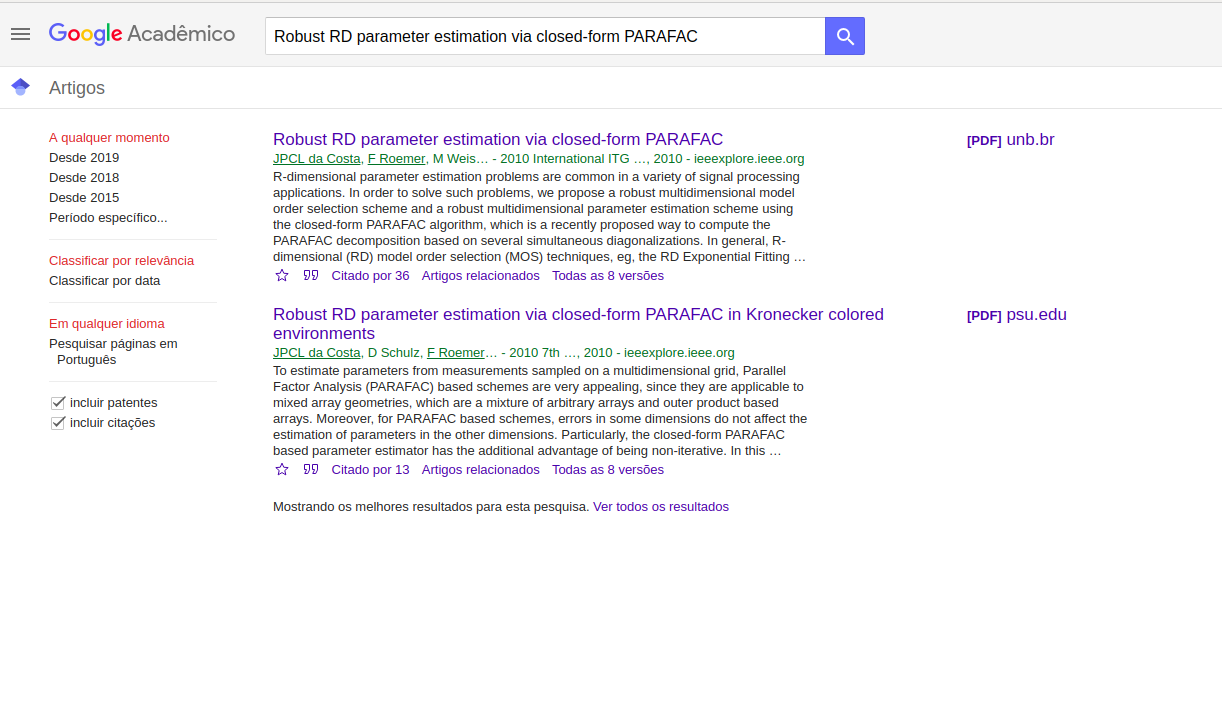
\includegraphics[width=0.6\textwidth]{figuras/google2.png}
	\caption{ }
\end{figure}
	
\begin{figure}[htbp!]
	\centering
	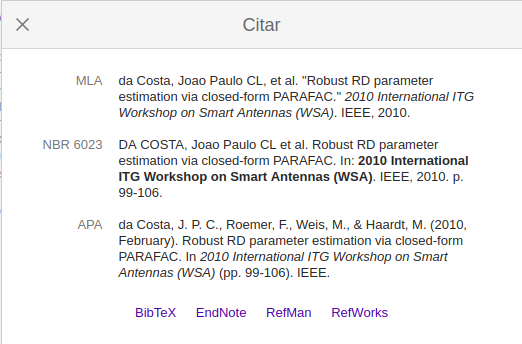
\includegraphics[width=0.4\textwidth]{figuras/google3.png}
	\caption{ }
\end{figure}
\end{multicols}
\end{frame}
	


\input{glossaries/glosarie}

\section{Tikz} % (fold)
\label{sec:tikz}

\begin{frame}{O que é?}
\begin{block}{}
	\begin{itemize}
		\item Um dos melhores pacotes para {\bf produzir} gráficos \underline{vetorizados} em \LaTeX.
		\item Possui um extensa \href{http://ftp.fau.de/ctan/graphics/pgf/base/doc/pgfmanual.pdf}{documentação}.
		\item Disponibiliza diversos \href{http://www.texample.net/tikz/examples/}{exemplos} de como utilizar o pacote.
	\end{itemize}
\end{block}
\end{frame}

\subsection*{Vantagens \& Desvantagens}
\begin{frame}{Vantagens}
	\begin{multicols}{2}		
	\input tikz/gnuplot
	\input tikz/polar
	\end{multicols}
\end{frame}

% section tikz (end)
\begin{frame}{Vantagens}
	\begin{multicols}{2}		
	\input tikz/square
	\input tikz/circuitikz
	\end{multicols}
\end{frame}

\begin{frame}{Vantagens}	
	\input tikz/neural
\end{frame}


\begin{frame}{Desvantagens}
	\begin{block}{}
		\begin{itemize}
			\item Péssima curva de aprendizado.
			\item Desalinhamento de  versões entre o disponibilizado nos repositórios com os apresentados nos exemplos.
			\item {\it Sujo}
		\end{itemize}
	\end{block}
\end{frame}

\subsection*{Exemplos}
\begin{frame}{Circuito}
	\lstinputlisting[linewidth=8cm,basicstyle=\tiny\ttfamily]{tikz/circuitikz.tex}
\end{frame}

\begin{frame}{GnuPlot}
	\lstinputlisting[linewidth=8cm,basicstyle=\tiny\ttfamily]{tikz/gnuplot.tex}
\end{frame}

\begin{frame}[shrink=30]{Neural Network}
	\lstinputlisting[linewidth=8cm,basicstyle=\tiny\ttfamily]{tikz/neural.tex}
\end{frame}

\section*{}
\begin{frame}
\begin{center}
  \Huge\ttfamily \textbf {OBRIGADO!}
\end{center}
\end{frame}


\end{document}
